\section{Materiales y métodos}

\subsection{Materiales}
Los genes relacionados con el fenotipo ``Maternal diabetes'' (HP:0009800) fueron extraídos de la base de datos Human Phenotype Ontology (HPO) en la web hpo.jax \cite{Kohler2017}. Específicamente, se trabajó con una lista de 43 genes asociados al fenotipo, la cual se encontraba en formato .xlsx.

Se utilizaron las librerías de Python
openpyxl 3.1.2, Stringdb 0.1.5 \cite{Mering2005}, Pandas 2.1.2 \cite{McKinney2015}, iGraph 0.11.2 \cite{Csardi2006} y Cairocffi 1.6.1, para el procesamiento de datos y las representaciones.

Los scripts se han ejecutado en un MacBook Air 15 con Intel Core i5-5250U CPU 1.60GHz, 8 GB RAM y sistema operativo Ubuntu 22.04.3 LTS (Jammy Jellyfish).

\subsection{Metodología}

El flujo de trabajo que se siguió puede observarse en la figura \ref{fig:workflow} y se explicará en detalle a continuación.

\begin{figure}[h!]
	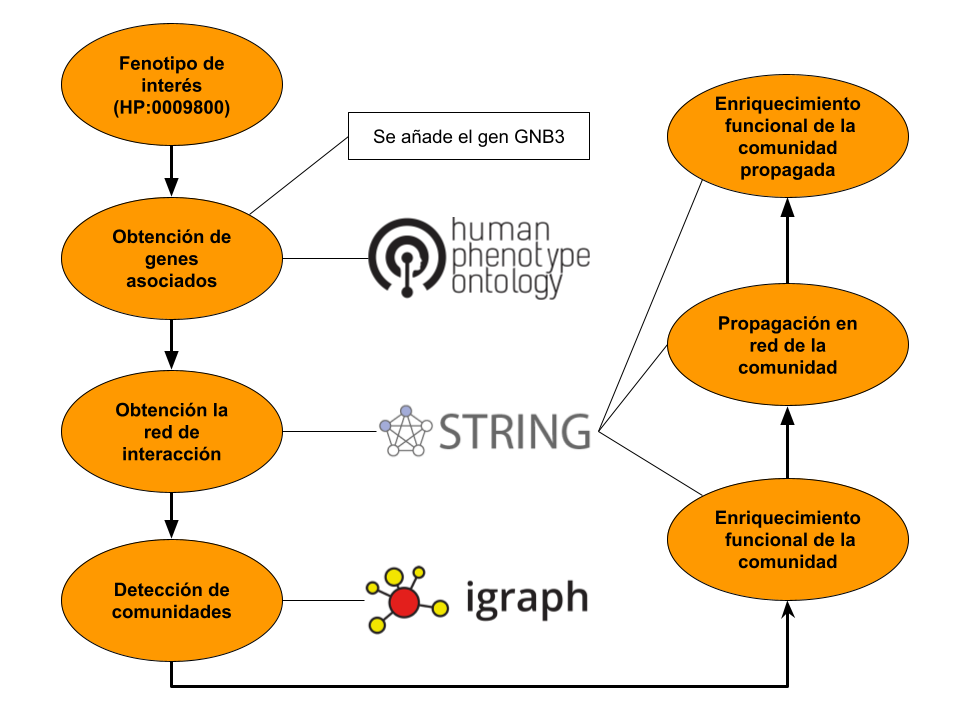
\includegraphics[width=0.9\textwidth]{figures/workflow.png}
	\caption{Flujo de trabajo: Se representa el flujo de trabajo seguido para la realización del proyecto. Empieza desde la obtención de los genes asociados al fenotipo de interés y la creación de la red de interacción hasta el análisis por enriquecimiento funcional.}
	\label{fig:workflow}
\end{figure}

Descargamos la lista de genes implicados al fenotipo HP:0009800 directamente desde HPO en formato xlsx e insertamos en la lista el gen GNB3 (id = 2784).

Utilizamos la librería Stringdb de Python para obtener la red de interacción de los genes asociados al fenotipo, su cantidad de nodos y enlaces. También fue obtenida la red de interacción de los genes asociados junto con el gen GNB3.

Mediante la librería de iGraph se construyó la red de interacción de genes y se realizó un algoritmo de detección de comunidades basado en ``edge betweenness'' \cite{Girvan2002}, también conocido como intermediación de aristas. Esta métrica evalúa la influencia de un nodo sobre el flujo de información entre otros nodos  \cite{Girvan2002}. Para encontrar qué aristas de una red están más entre otros pares de vértices, se define la intersección de una arista como el número de trayectorias más cortas entre los pares de vértices que corren a lo largo de ella. En cada paso del algoritmo se elimina la arista con menos intermediación  \cite{Girvan2002}. Una vez realizada la detección, se seleccionó la comunidad donde estaba presente el gen GNB3.

Realizamos un enriquecimiento funcional \cite{Chicco2022}, técnica que identifica las vías biológicas más sobrerrepresentadas en una lista de genes en comparación con las que se asociarían a ellos por azar, de los genes que formaban parte de esa comunidad con la librería de Stringdb y filtramos el resultado para quedarnos con las filas donde aparece el gen GNB3. El enriquecimiento funcional fue hecho con el método ``get\_enrichment" de la librería mencionada, que devuelve las vías enriquecidas, sus términos, categoría y  valores como el p-valor y la tasa de descubrimiento falso (FDR) . Entre las categorías, destacamos Reactome (RCTM), que es una base de datos de vías biológicas \cite{Gillespie2021} y la categoría HPO \cite{Kohler2017} descrita en la sección de materiales.

Se creó una nueva red mediante una propagación en red de los genes presentes en la comunidad de interés, utilizando el método ``get\_network" del paquete Stringdb con el parámetro ``add\_nodes = 16'', que añade nodos basándose en medidas de confianza. A partir de esta red volvimos a realizar un enriquecimiento funcional.